\documentclass[12pt]{article}%
\usepackage{amsfonts}
\usepackage{fancyhdr}
\usepackage{comment}
\usepackage[a4paper, top=2.5cm, bottom=2.5cm, left=2.2cm, right=2.2cm]%
{geometry}
\usepackage{times}
\usepackage{amsmath}
\usepackage{changepage}
\usepackage{amssymb}
\usepackage{graphicx}%
\usepackage{wrapfig}
\setcounter{MaxMatrixCols}{30}
\newenvironment{proof}[1][Proof]{\textbf{#1.} }{\ \rule{0.5em}{0.5em}}

\newcommand{\Q}{\mathbb{Q}}
\newcommand{\R}{\mathbb{R}}
\newcommand{\C}{\mathbb{C}}
\newcommand{\Z}{\mathbb{Z}}

\begin{document}

\title{Information Visualization : Mobility in Brussels}
\author{Bruno M. Cabral, Pierre Gerard, Titouan Christophe, Luiz N. Junior}
\date{Vrije Universiteit Brussel}
\maketitle


\section{Introduction}
The mobility and public transportation in Brussels has a great importance in daily life of people using it.  Brussels region public transportation is organized into a vast number of lines that are divided into metro, tramways and buses, so the system is quite susceptible to suffer with exceptional events that happen in the city, which many times cause delays on its lines schedules, consequently, affecting its users.

The main goal of the project is trying to answer two questions which are related to this context of mobility via information visualization:

\begin{itemize}
	\item Is it possible to visualize the impact of street works or special events on brussels public transports ?
	\item Are there areas in the city that are significantly less served by public transports ?
\end{itemize}


\section{Data sources}
Some external different data sets were used in order to help supporting answering those questions. 

\subsection{Public Transportation Stops}

The public transportation network on Brussels region is managed by Brussels Intercommunal Transport Company (STIB/MIVB). The dataset used providing all stops locations (coordinates) is available at Open Data Brussels web portal % reference needed

\subsection{Lines Itineraries}

Information related to the itineraries of the lines - the sequence of stops that the lines passes by - and the time schedule to each stop were scraped from STIB/MIVB web portal, but it was already available in relational database.

\subsection{Delay events}
Data related to delay events that affects public transports lines are retrieved parsing information given by the official twitter of STIB/MIVB. % reference needed
That was possible due the fact that the published tweets follows an standard for the use of hashtags
Some specifics period events that happened in the city in the last months were added manually to the application, i.e. The european summit that happened in March.                       
                       
\section{Architecture}
We mostly used web technologies to create our visualization.

\subsection{Front-end}
% bootstrap, leaflet, d3, es , npm
% main challenge ? getting npm to work like we wanted ? 

\subsection{Back-end}
% flask, postgresql
 
\section{The visualization}

\subsection{Modal}

To ease the way for users unfamiliar with the visualization, we created a modal. That is a documentation page overlaying the visualization itself providing guidance to the user. That idea come from other visualization found on the web (eg : World Atlas of Language Structures \cite{visuawithmodal}).

\subsection{Map view}

\subsubsection{Stop density}


\subsubsection{Lines}

\subsection{Detailed view}

% Wrapping a figure does not want to work

%\begin{wrapfigure}{l}{0.35\textwidth}
%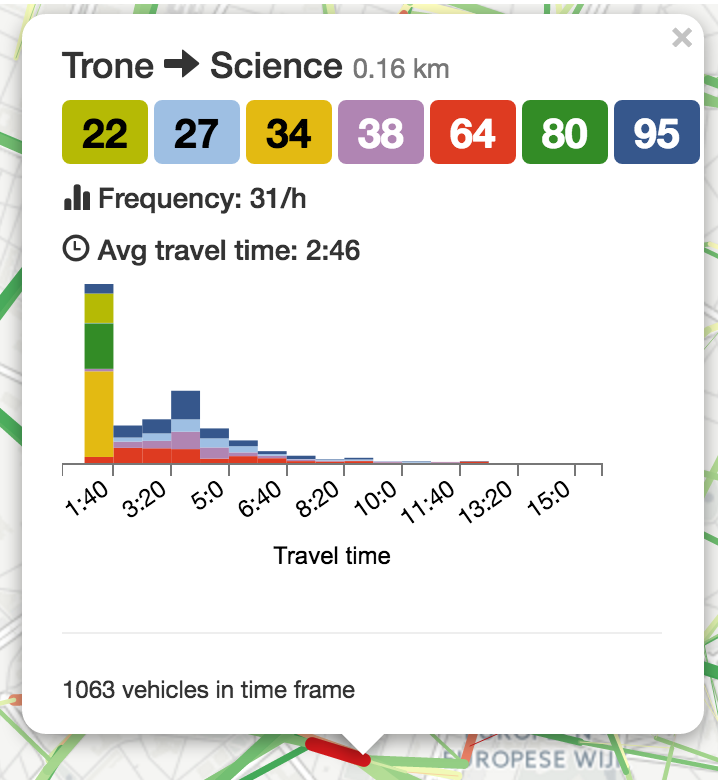
\includegraphics[width=0.95\linewidth]{images/tooltip.png} 
%\label{fig:subim1}
%\end{wrapfigure}

%Clicking on a line open a tooltip offering detailed information about the line.

%\textbf{Ah ha!} On the image on the left, we can this that between Trone and Science, the 22 and 34 bus are going faster than the other

%\vspace{6 cm}

\subsection{Events and time selection}

\section{Acknowledgement}

We would like to thanks Nikita Marchant and it's STIB data project \cite{nikita} project which enables us to get the delay data in the form of a postgresql relational database.

\section{Conclusion}


 
\begin{thebibliography}{9}
%\bibitem{nikita} 
%Michel Goossens, Frank Mittelbach, and Alexander Samarin. 
%\textit{The \LaTeX\ Companion}. 
%Addison-Wesley, Reading, Massachusetts, 1993.
 
\bibitem{nikita} 
Nikita Marchant: STIB scraper and delay prediction,
\\\texttt{https://github.com/C4ptainCrunch/info-f-308}

\bibitem{visuawithmodal} 
World Atlas of Language Structures,
\\\texttt{http://snip.ly/pJsZ#http://www.puffpuffproject.com/languages.html}



\end{thebibliography}

\end{document}